%%%%%%%%%%%%%%%%%%%%%%%%%%%%%%%%%%%%%%%%%%%%%%%%%%%%%%%%%%%%%%%%%%%%%%%
%% Document: Thesis for PhD at UC Riverside                          %%
%% Description: A comparative analysis of environment sensing in EDF %%
%% Author: Steven Ahrendt                                            %%
%%%%%%%%%%%%%%%%%%%%%%%%%%%%%%%%%%%%%%%%%%%%%%%%%%%%%%%%%%%%%%%%%%%%%%%
% COELOMOMYCES FIGURES %
%%%%%%%%%%%%%%%%%%%%%%%%
% GO-slim plot
\begin{figure}[hb]
  \centering
  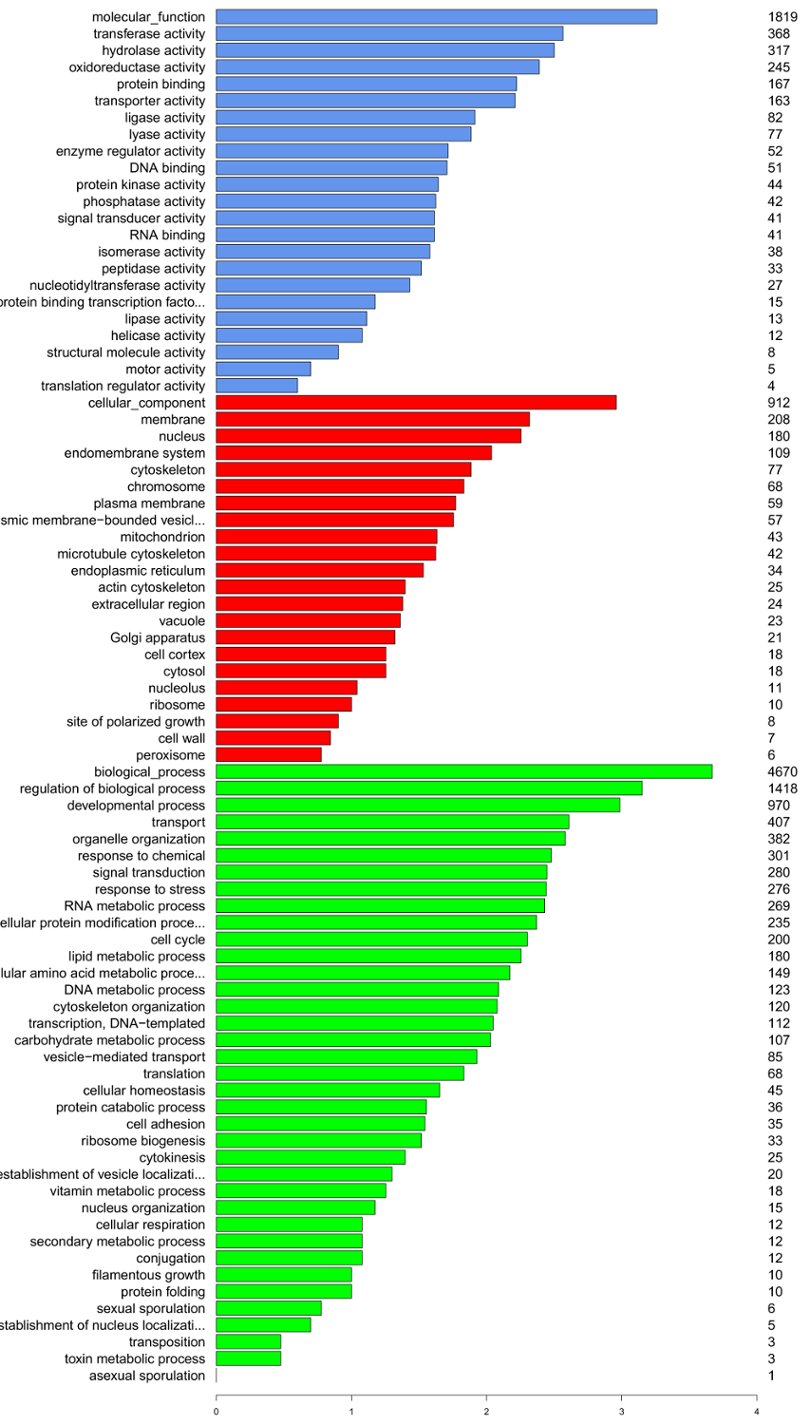
\includegraphics[width=4in]{./Chapter_Coelomomyces/img/Clat_aspergillus_GOPlot.png}
  \caption[\textit{C. lat} transcriptome GO term distribution]{Horizontal bar chart showing the distribution of \textit{Aspergillus} GO-Slim terms associated with the \textit{C. lativitattus} transcriptome. X axis is a logarithmic scale.}
  \label{fig:ChClat_GOPlot}
\end{figure}

% Opsin-GC fusion; chytrid cluster
\begin{figure}[hb]
  \centering
  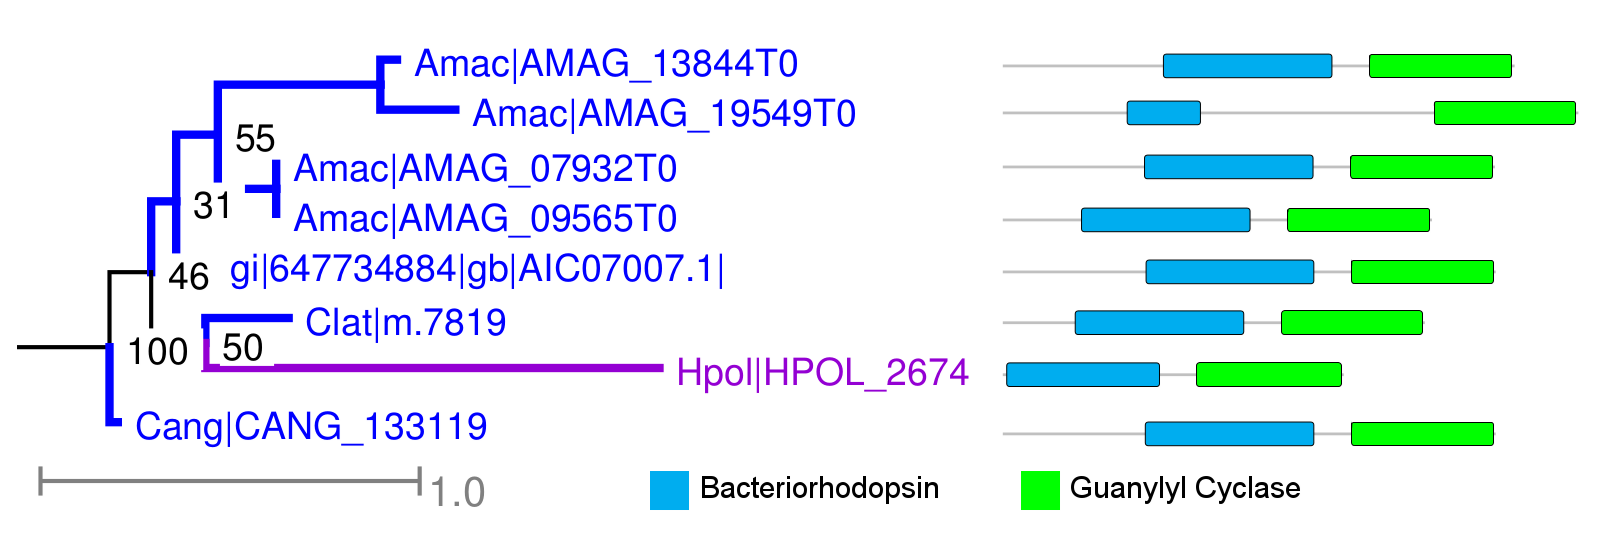
\includegraphics[width=4in]{./Chapter_Coelomomyces/img/OpsinGCFusion_chytridCluster.png}
  \caption[Opsin-GC fusion proteins]{A subset of bacterial opsin-guanylate cyclase fusion proteins. Proteins with similar architecture as described for \textit{B. emersonii} identified in Blastocladiomycete and Chytridiomycete proteomes, and \textit{C. lativitattus} transcriptome.}
  \label{fig:ChClat_OpsinGC}
\end{figure}

% Beta-carotene distribution
\begin{figure}[hb]
  \centering
  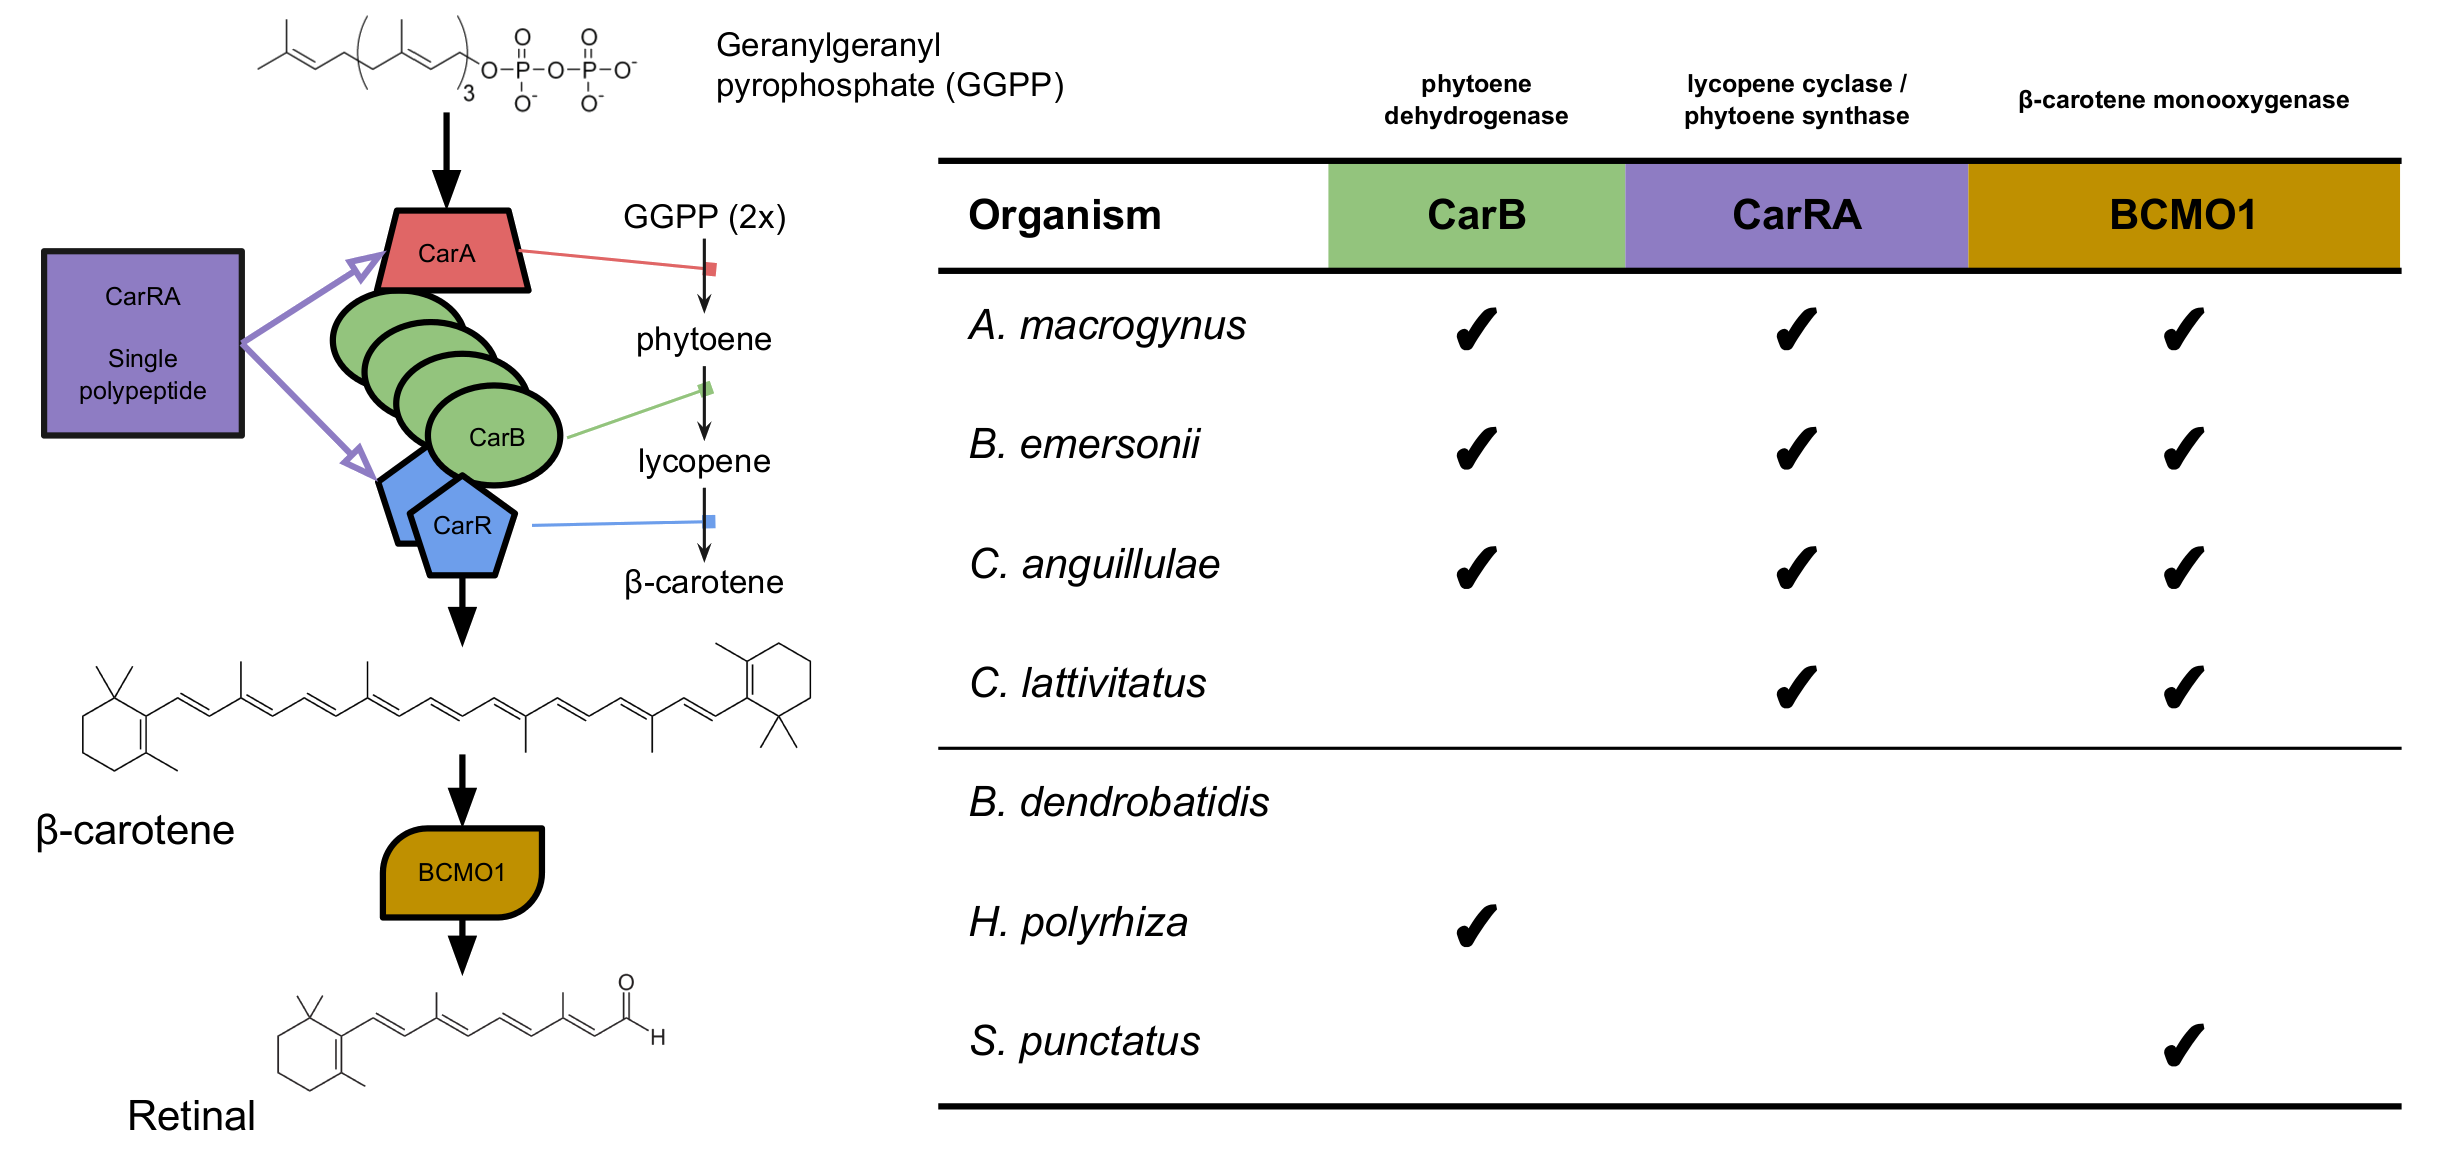
\includegraphics[width=4in]{./Chapter_Coelomomyces/img/Figure_bcaroPresenceAbsence.png}
  \caption[$\beta$-carotene enzyme presence / absence]{Presence and absence of $\beta$-carotene related proteins in species belonging to the Chytridiomycota and Blastocladiomycota.}
  \label{fig:ChClat_Bcaro}
\end{figure}

% PF00112 tree
\begin{figure}[hb]
  \centering
  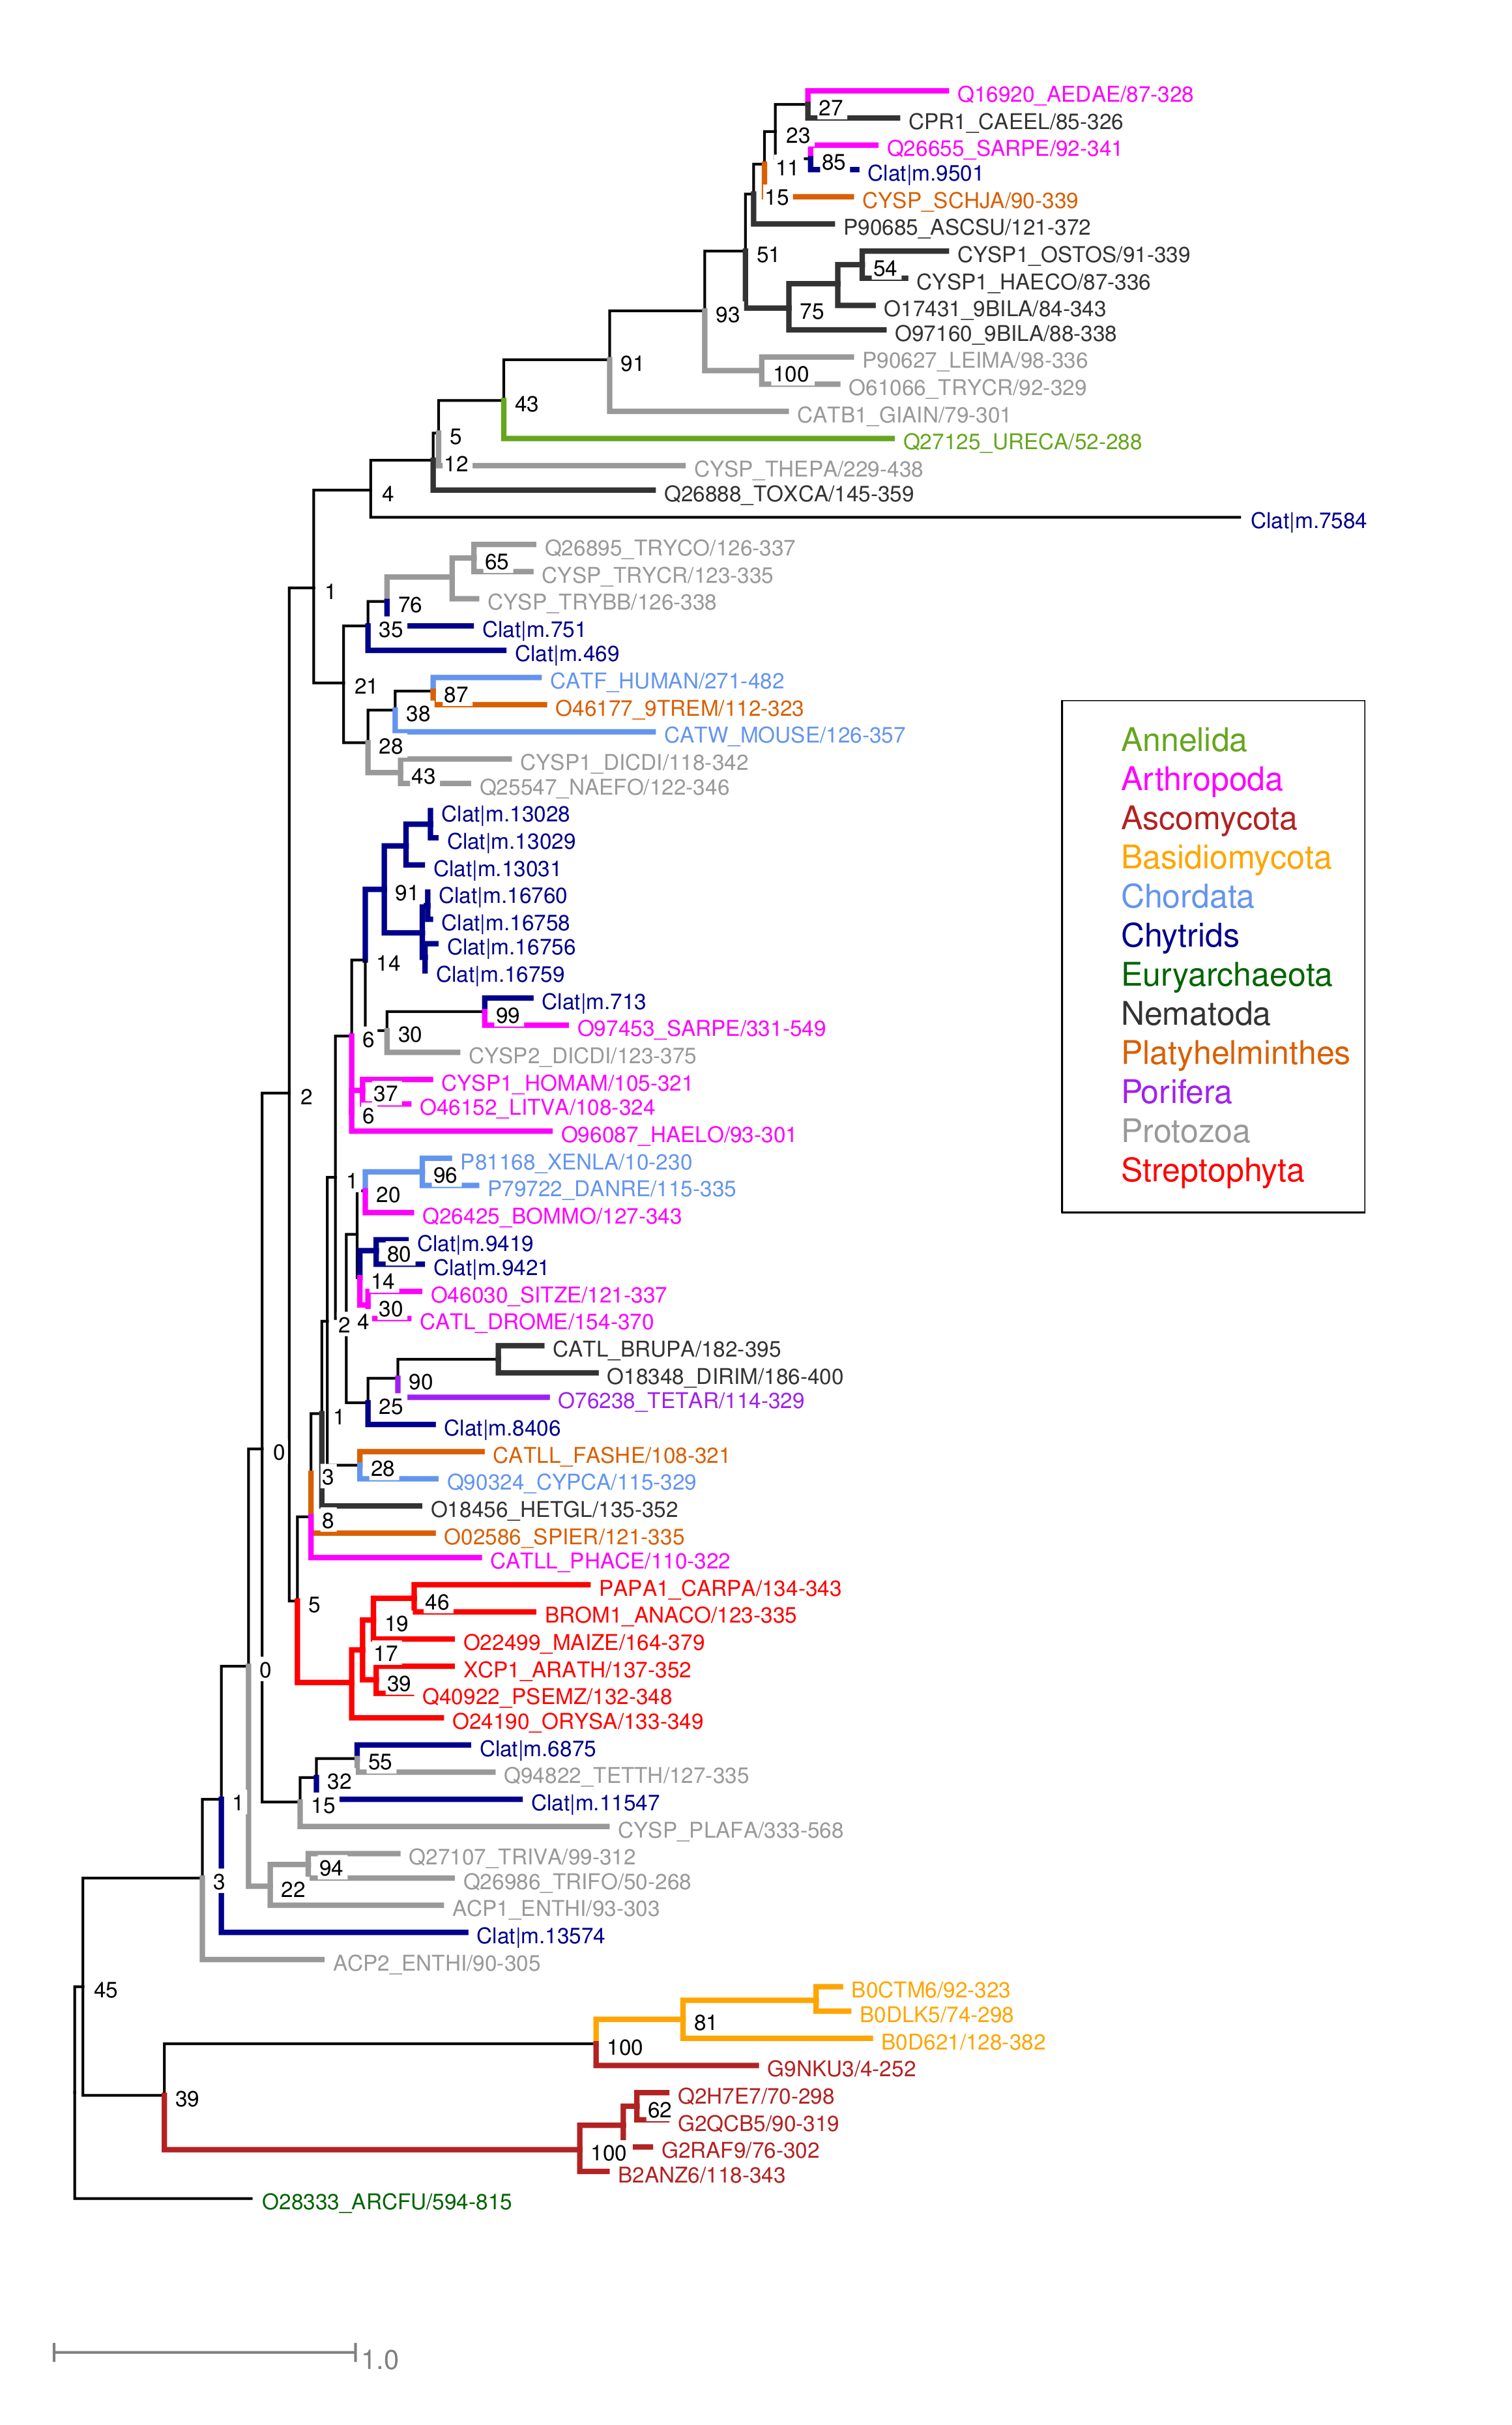
\includegraphics[width=4in]{./Chapter_Coelomomyces/img/PF00112_tree.png}
  \caption[PF00112 RAxML tree]{RAxML tree of select PF00112 seed sequences, unique \textit{C. lat} protein sequences, and sequences from Dikarya species.}
  \label{fig:ChClat_PF00112}
\end{figure}

% PF00089 tree
\begin{figure}[hb]
  \centering
  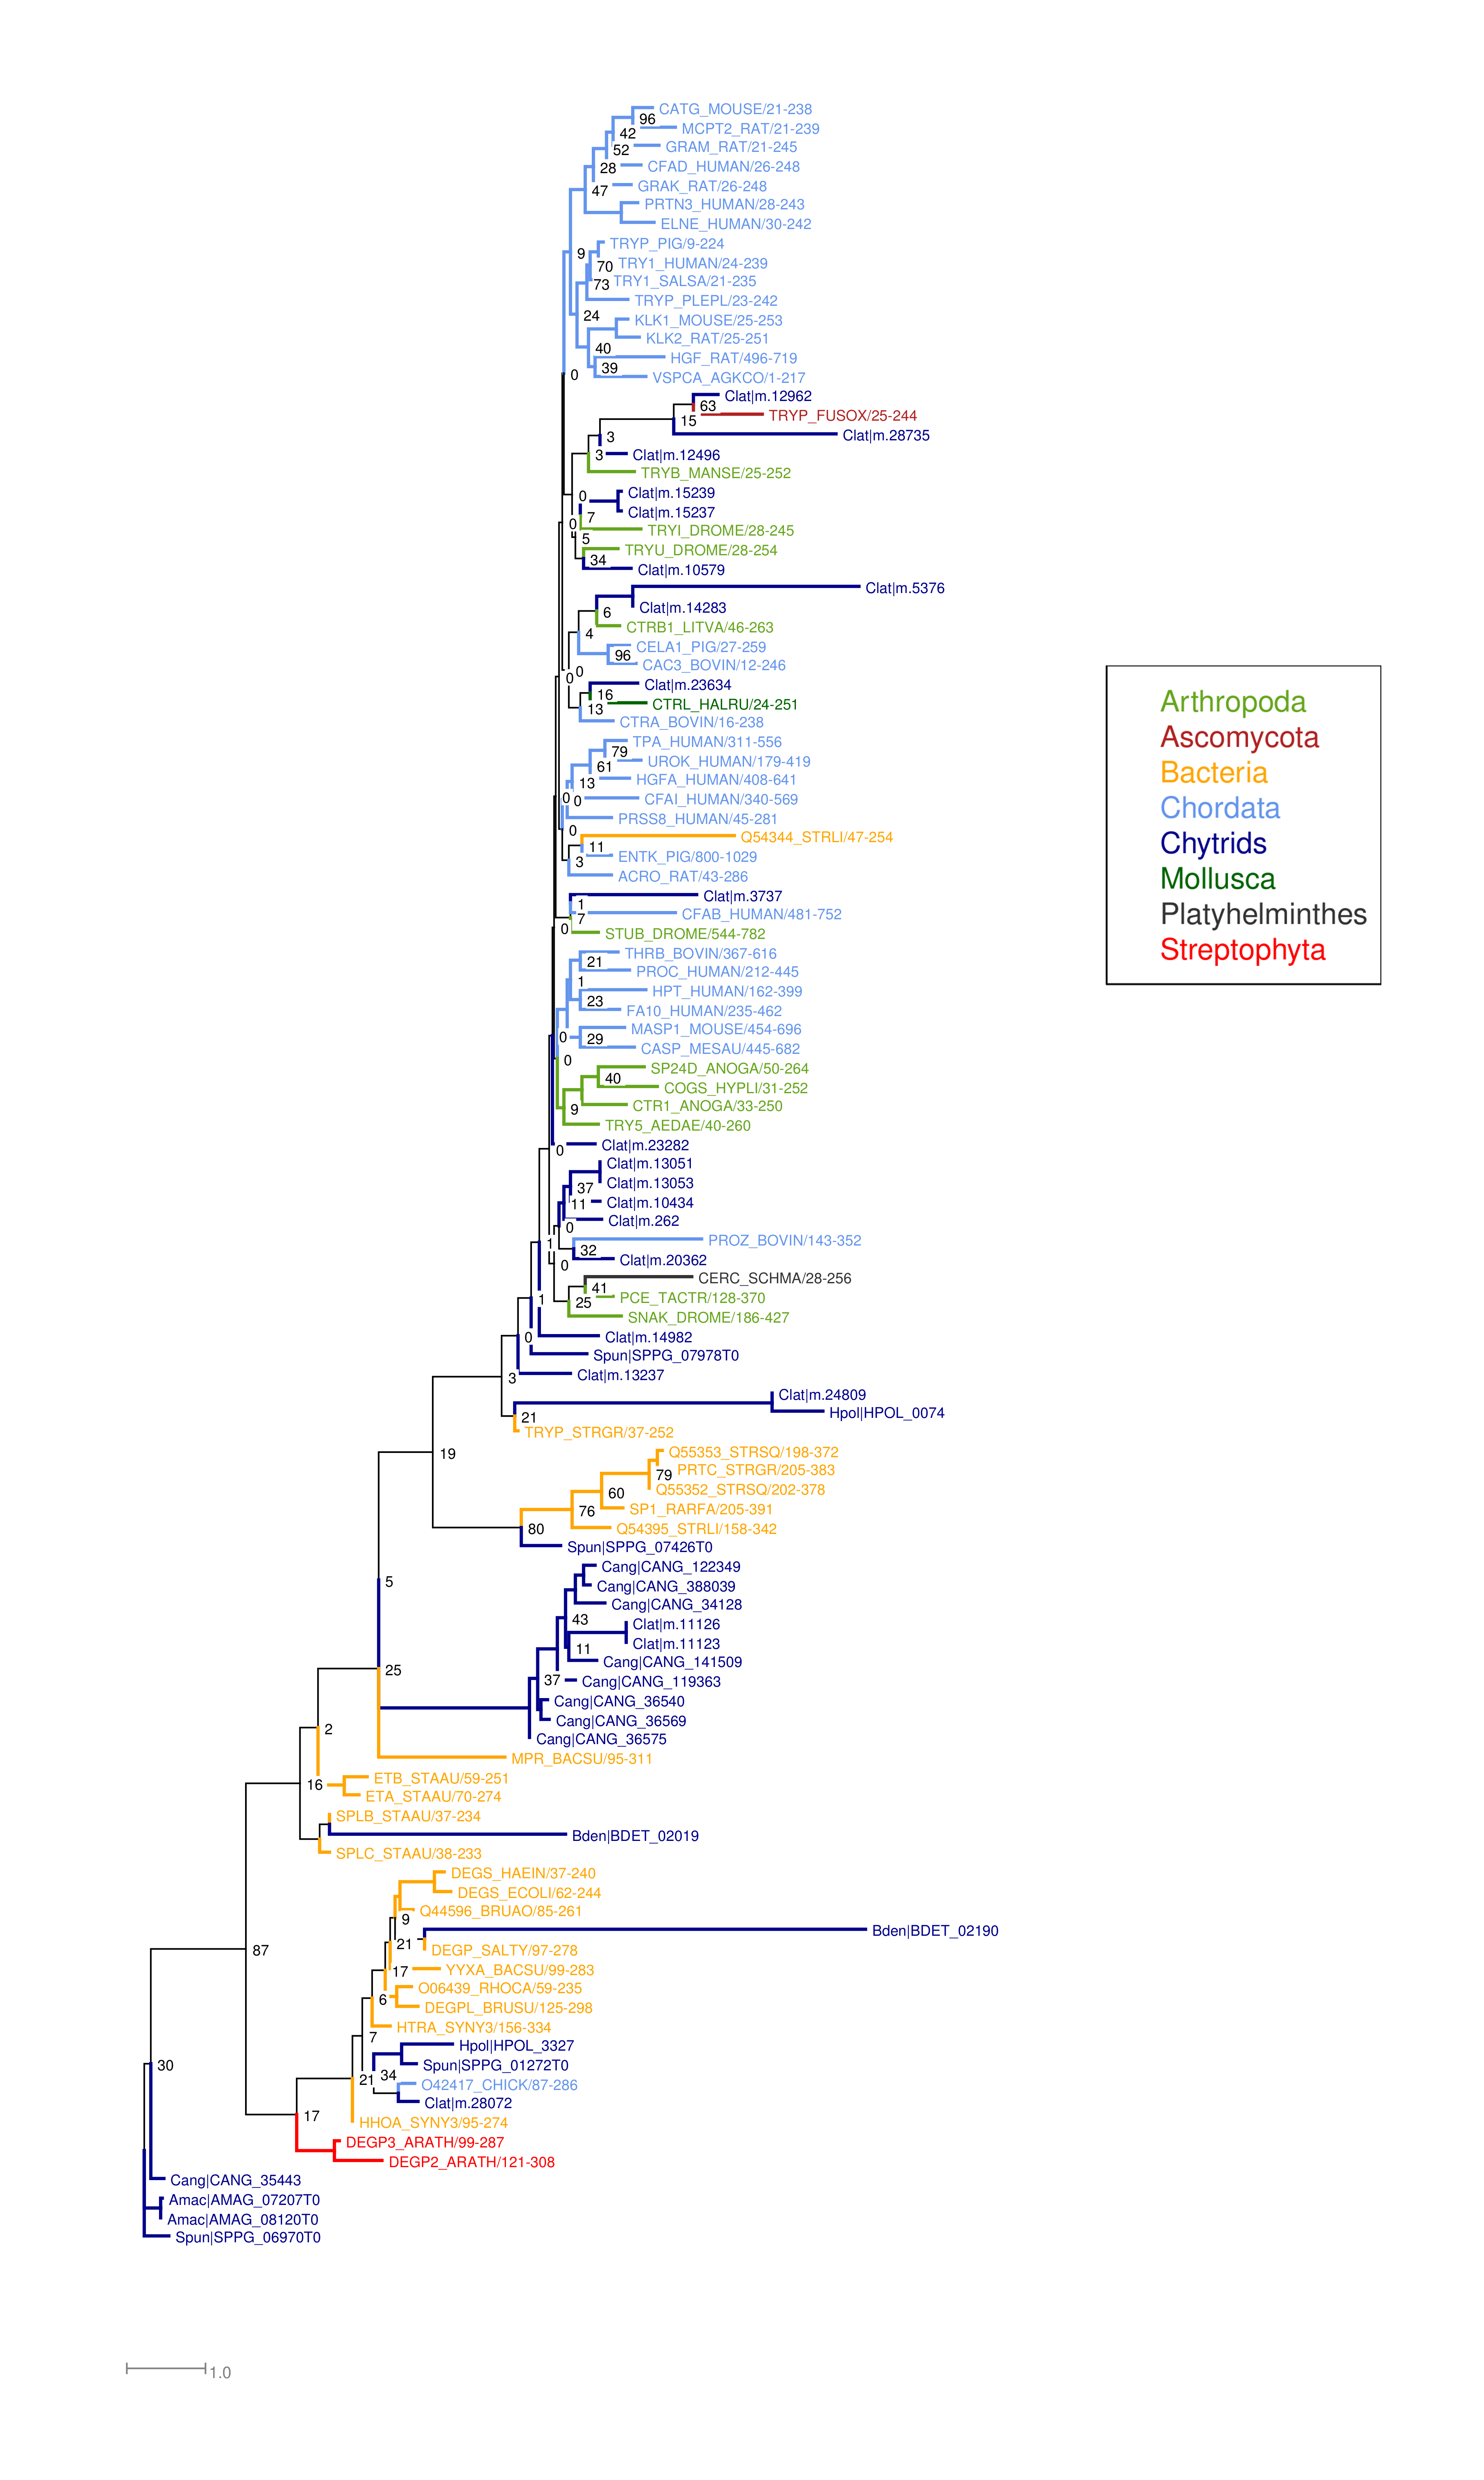
\includegraphics[width=4in]{./Chapter_Coelomomyces/img/PF00089_tree.png}
  \caption[PF00089 RAxML tree]{RAxML tree of select PF0089 seed sequences and unique \textit{C. lat} protein sequences}
  \label{fig:ChClat_PF00089}
\end{figure}

% 20HE receptor alignment
\begin{figure}[hb]
  \centering
  \begin{texshade}{./Chapter_Coelomomyces/dat/20HE_alignment.fa_aln}
    \threshold[80]{50}
    \shadingmode[allmatchspecial]{similar}
    \setends{1}{1..300}
    \hideconsensus
  \end{texshade}
  \caption[20HE alignment]{Alignment of \textit{D. melanogaster} EcR and putative 20HE receptors identified in \textit{C. lativittatus} }
  \label{fig:ChClat_20HEalign}
\end{figure}
